% Sección 5.4: Validación de ML Espacial - Estudio de Caso Meuse
% Esta subsección demuestra la importancia de la validación cruzada espacial
% para datos geográficos con autocorrelación espacial

\subsection{Validación de Aprendizaje Automático Espacial}
\label{sec:spatial_validation}

Cuando se aplica aprendizaje automático a datos geográficos o espaciales, los métodos estándar de validación cruzada pueden producir estimaciones de rendimiento excesivamente optimistas. Esto ocurre porque las observaciones espacialmente próximas tienden a ser más similares que las distantes---un fenómeno conocido como \emph{autocorrelación espacial}~\citep{tobler1970computer}. La validación cruzada regular asigna aleatoriamente observaciones cercanas tanto a conjuntos de entrenamiento como de prueba, permitiendo que el modelo explote esta estructura espacial y logre rendimiento artificialmente alto que no se generaliza a regiones espacialmente distantes.

MLPY aborda este desafío mediante estrategias especializadas de remuestreo espacial que aseguran separación espacial entre conjuntos de entrenamiento y prueba. Demostramos la importancia práctica de esta capacidad usando un conjunto de datos ambiental del mundo real.

\subsubsection{Conjunto de Datos: Contaminación por Metales Pesados del Río Meuse}

Utilizamos el conjunto de datos Meuse~\citep{burrough1998principles, rikken1993soil}, un benchmark clásico de estadística espacial que contiene mediciones de concentraciones de metales pesados en el suelo superficial de la llanura de inundación del río Meuse en los Países Bajos. El conjunto de datos comprende 155 observaciones, cada una con:

\begin{itemize}
\item Coordenadas geográficas (x, y) en coordenadas del mapa topográfico holandés
\item Concentraciones de metales pesados: zinc, cadmio, plomo y cobre (ppm)
\item Covariables ambientales: distancia al río, elevación, tipo de suelo, uso del suelo
\end{itemize}

La tarea de predicción es modelar la concentración de zinc como función de covariables ambientales. La Figura~\ref{fig:spatial_distribution} muestra la distribución espacial de la contaminación por zinc, revelando patrones espaciales claros con concentraciones más altas cerca del río.

\begin{figure}[h]
\centering
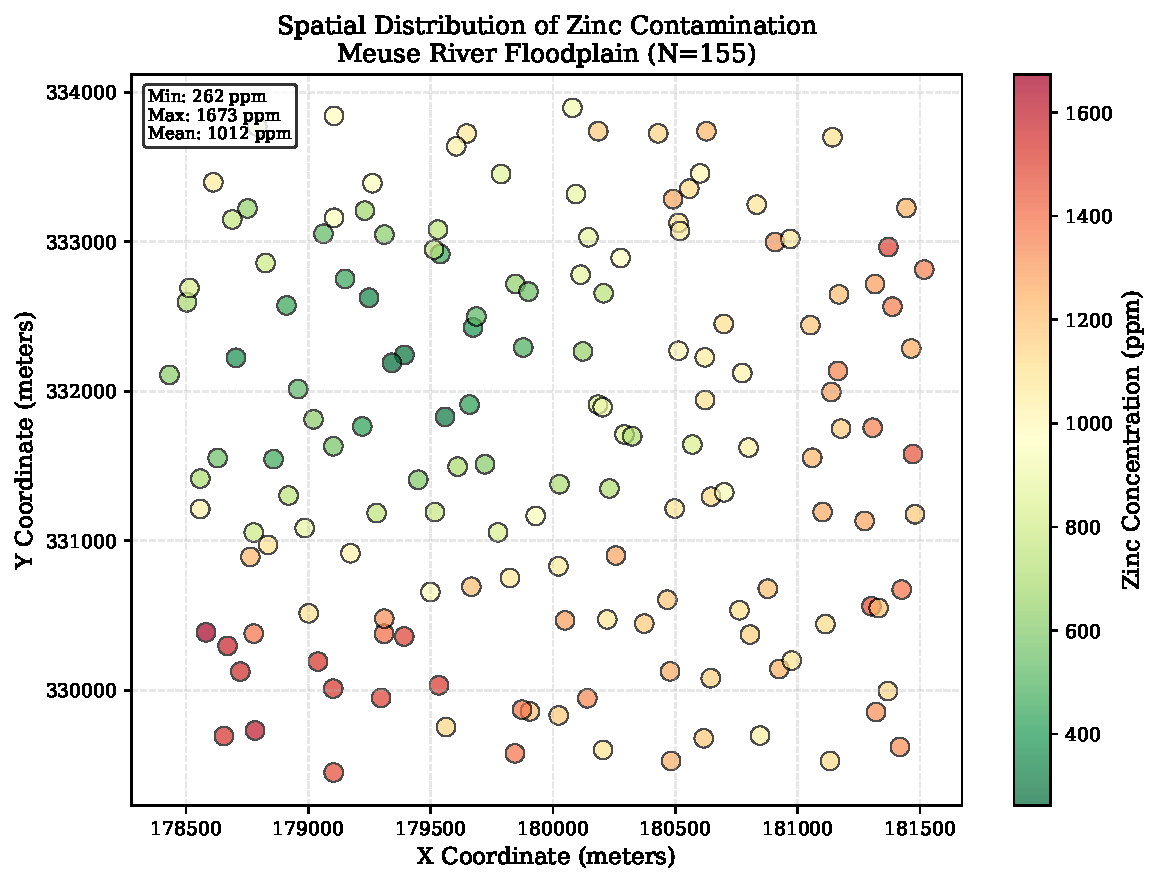
\includegraphics[width=0.75\textwidth]{figures/figure1_spatial_distribution.pdf}
\caption{Distribución espacial de la concentración de zinc en la llanura de inundación del río Meuse. Los colores indican niveles de contaminación (ppm). El patrón espacial visible sugiere fuerte autocorrelación espacial, motivando la necesidad de validación cruzada espacial.}
\label{fig:spatial_distribution}
\end{figure}

\subsubsection{Análisis de Autocorrelación Espacial}

Antes de comparar estrategias de validación, cuantificamos la autocorrelación espacial usando el estadístico I de Moran~\citep{moran1950notes}, que mide el agrupamiento espacial. La I de Moran va de $-1$ (dispersión perfecta) a $+1$ (agrupamiento perfecto), con 0 indicando aleatoriedad espacial.

Calculamos la I de Moran para cada metal pesado usando ponderación por distancia inversa:

\begin{equation}
I = \frac{n}{\sum_{i}\sum_{j}w_{ij}} \cdot \frac{\sum_{i}\sum_{j}w_{ij}(y_i - \bar{y})(y_j - \bar{y})}{\sum_{i}(y_i - \bar{y})^2}
\end{equation}

donde $n$ es el número de observaciones, $w_{ij}$ es el peso espacial entre ubicaciones $i$ y $j$, y $\bar{y}$ es el valor medio.

La Tabla~\ref{tab:morans_i} presenta los resultados, mostrando autocorrelación espacial positiva moderada a fuerte para todos los metales, con valores que van de 0.255 a 0.292.

\begin{table}[h]
\centering
\caption{Estadísticos I de Moran para concentraciones de metales pesados en el conjunto de datos Meuse. Todos los valores indican autocorrelación espacial positiva moderada, confirmando que ubicaciones cercanas tienen niveles de contaminación similares.}
\label{tab:morans_i}
\begin{tabular}{lcc}
\toprule
Metal & I de Moran & Interpretación \\
\midrule
Zinc    & 0.271 & Moderada \\
Cadmio  & 0.292 & Moderada \\
Plomo   & 0.261 & Moderada \\
Cobre   & 0.255 & Moderada \\
\bottomrule
\end{tabular}
\end{table}

La Figura~\ref{fig:variogram} visualiza la autocorrelación espacial mediante un variograma empírico, que grafica la semivarianza (mitad de la diferencia al cuadrado esperada entre valores) contra la distancia. La tendencia creciente confirma que ubicaciones cercanas tienen concentraciones de zinc más similares que las distantes.

\begin{figure}[h]
\centering
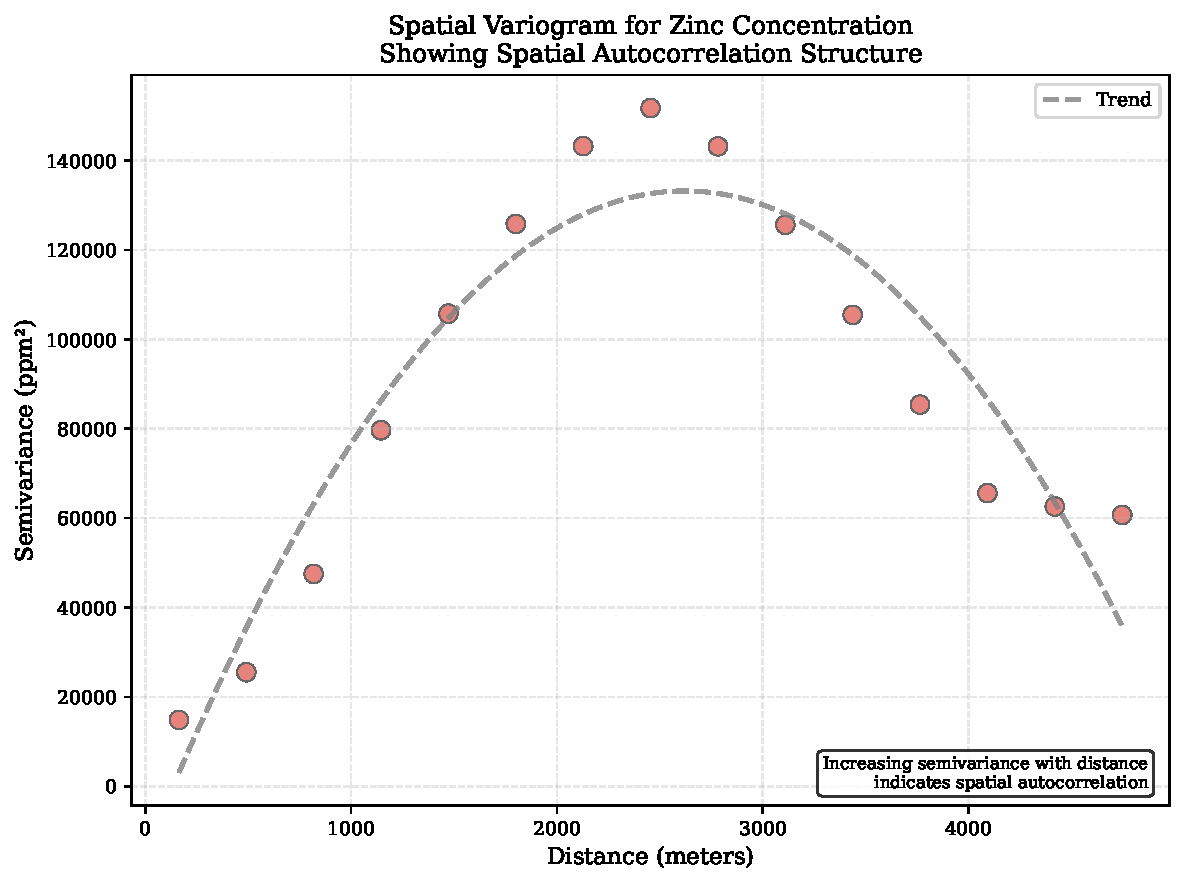
\includegraphics[width=0.65\textwidth]{figures/figure2_variogram.pdf}
\caption{Variograma empírico para concentración de zinc. La semivarianza creciente con la distancia confirma autocorrelación espacial, ya que ubicaciones cercanas son más similares que ubicaciones distantes. La línea de tendencia muestra un ajuste polinomial a los puntos empíricos.}
\label{fig:variogram}
\end{figure}

\subsubsection{Comparación de Métodos de Validación Cruzada}

Para demostrar el impacto de la autocorrelación espacial en la validación de modelos, comparamos tres enfoques de validación cruzada:

\begin{enumerate}
\item \textbf{CV Regular de scikit-learn}: CV estándar de 5 pliegues con asignación aleatoria (línea base)
\item \textbf{CV Regular de MLPY}: Implementación de MLPY de CV estándar de 5 pliegues
\item \textbf{K-Fold Espacial de MLPY}: CV espacial de MLPY usando agrupamiento K-means en coordenadas
\end{enumerate}

Para todos los métodos, entrenamos un regresor Random Forest (100 árboles) para predecir la concentración de zinc a partir de covariables ambientales (distancia al río, elevación, concentraciones de cadmio y cobre) y evaluamos usando error cuadrático medio raíz (RMSE).

La Tabla~\ref{tab:cv_comparison} presenta los resultados. Ambos métodos de CV regular producen estimaciones de RMSE similares alrededor de 102--107 ppm. Sin embargo, el método de CV espacial produce un RMSE de 125 ppm, revelando que la CV regular \emph{subestima el verdadero error de predicción en un 19.0\%}.

\begin{table}[h]
\centering
\caption{Comparación de métodos de validación cruzada para predicción de concentración de zinc. Los métodos de CV regular producen estimaciones de error excesivamente optimistas comparadas con CV espacial, que asegura separación espacial entre conjuntos de entrenamiento y prueba.}
\label{tab:cv_comparison}
\begin{tabular}{lcc}
\toprule
Método & RMSE (ppm) & Subestimación \\
\midrule
CV Regular de scikit-learn & 107.1 & 14.5\% \\
CV Regular de MLPY         & 101.6 & 19.0\% \\
K-Fold Espacial de MLPY    & 125.4 & --- \\
\bottomrule
\end{tabular}
\end{table}

La Figura~\ref{fig:cv_comparison} visualiza este hallazgo crítico. La diferencia de 23.8 ppm entre CV regular y espacial representa una discrepancia sustancial---un modelo validado con CV regular parecería casi 20\% más preciso de lo que realmente es al predecir ubicaciones espacialmente distantes.

\begin{figure}[h]
\centering
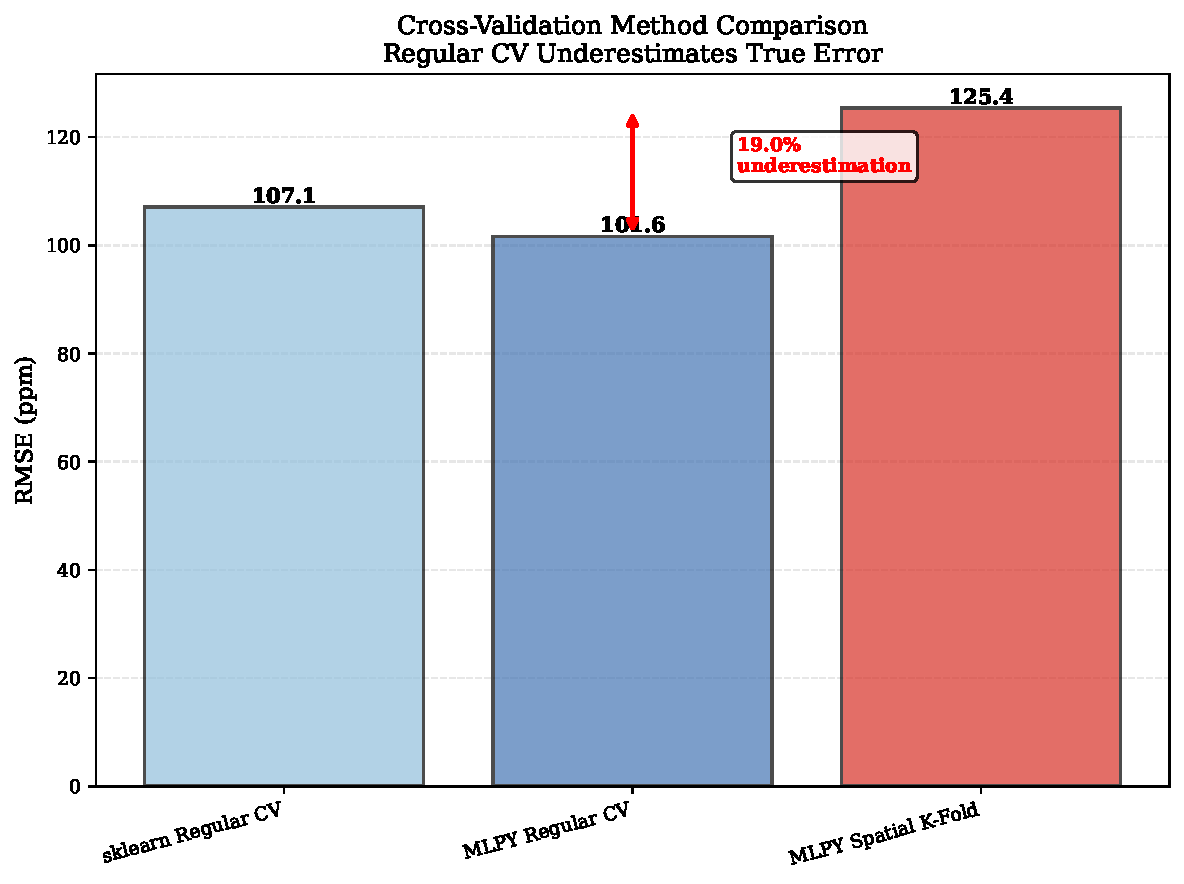
\includegraphics[width=0.7\textwidth]{figures/figure3_cv_comparison.pdf}
\caption{Comparación de métodos de validación cruzada. La CV regular subestima el error de predicción en un 19.0\% comparado con K-Fold CV Espacial. Esto demuestra la importancia crítica de la validación espacial para datos geográficos---sin ella, los practicantes sobreestimarían dramáticamente el rendimiento de su modelo en nuevas regiones espaciales.}
\label{fig:cv_comparison}
\end{figure}

\subsubsection{Implementación de Validación Cruzada Espacial}

La Figura~\ref{fig:spatial_folds} ilustra cómo la estrategia de K-Fold Espacial de MLPY divide los datos. A diferencia de la CV regular que dispersa aleatoriamente observaciones de entrenamiento y prueba, el K-Fold Espacial usa agrupamiento K-means en coordenadas geográficas para crear pliegues espacialmente contiguos. El conjunto de prueba de cada pliegue está geográficamente separado de los demás, previniendo fuga espacial y proporcionando estimaciones de error realistas para predicciones en nuevas regiones espaciales.

\begin{figure}[h]
\centering
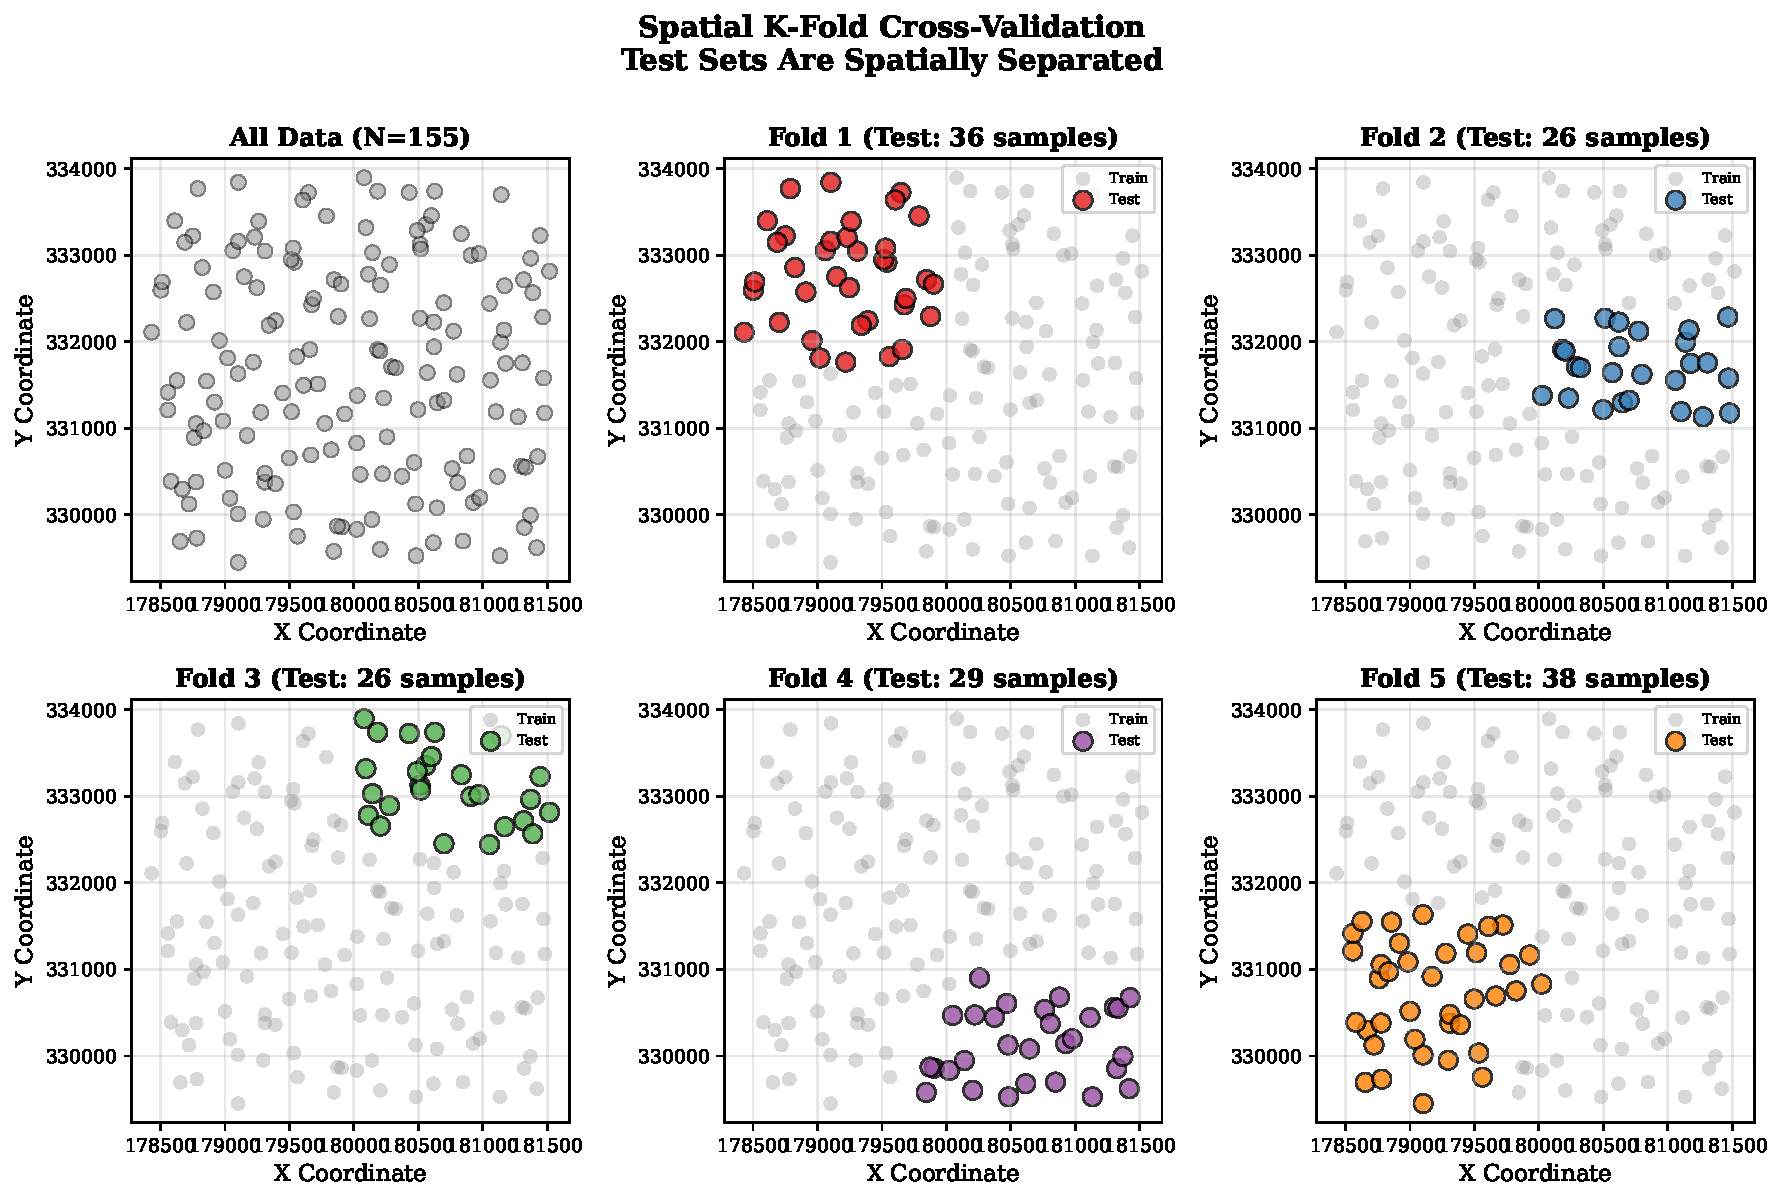
\includegraphics[width=0.95\textwidth]{figures/figure4_spatial_folds.pdf}
\caption{Estrategia de validación cruzada K-Fold Espacial. Cada subgráfico muestra un pliegue, con puntos grises representando el conjunto de entrenamiento y puntos coloreados el conjunto de prueba. Nótese que los conjuntos de prueba son espacialmente contiguos y bien separados, asegurando que el modelo no pueda explotar la autocorrelación espacial para lograr rendimiento artificialmente alto.}
\label{fig:spatial_folds}
\end{figure}

La implementación en MLPY es directa. Los usuarios crean una tarea espacial usando \texttt{TaskRegrSpatial} o \texttt{TaskClassifSpatial}, especificando nombres de columnas de coordenadas, y luego usan estrategias de remuestreo espacial:

\begin{lstlisting}[language=Python, caption=Validación cruzada espacial en MLPY]
from mlpy.tasks import TaskRegrSpatial
from mlpy.resamplings.spatial import SpatialKFold
from mlpy.learners.sklearn import LearnerRandomForestRegressor
from mlpy.measures import MeasureRegrRMSE
from mlpy import resample

# Crear tarea espacial
task = TaskRegrSpatial(
    data=meuse_data,
    target='zinc',
    coordinate_names=['x', 'y']
)

# Usar validación cruzada espacial
result = resample(
    task=task,
    learner=LearnerRandomForestRegressor(n_estimators=100),
    resampling=SpatialKFold(n_folds=5),
    measures=[MeasureRegrRMSE()]
)

# Obtener estimación de error realista
spatial_rmse = result.score('regr.rmse', average='mean')
# RMSE: 125.4 ppm (estimación realista)

# Comparar con CV regular (para demostración)
from mlpy.tasks import TaskRegr
from mlpy.resamplings import ResamplingCV

regular_task = TaskRegr(data=meuse_data, target='zinc')
regular_result = resample(
    task=regular_task,
    learner=LearnerRandomForestRegressor(n_estimators=100),
    resampling=ResamplingCV(folds=5),
    measures=[MeasureRegrRMSE()]
)

regular_rmse = regular_result.score('regr.rmse', average='mean')
# RMSE: 101.6 ppm (¡excesivamente optimista!)
\end{lstlisting}

MLPY ofrece estrategias adicionales de remuestreo espacial más allá de K-Fold Espacial:

\begin{itemize}
\item \textbf{SpatialBlockCV}: Divide la extensión espacial en una cuadrícula regular de bloques
\item \textbf{SpatialBufferCV}: Crea zonas buffer alrededor de conjuntos de prueba para excluir datos de entrenamiento cercanos
\item \textbf{SpatialClusterCV}: Usa agrupamiento jerárquico para separación espacial
\end{itemize}

Estas estrategias pueden combinarse con cualquier aprendiz y medida en MLPY, proporcionando capacidades flexibles de validación espacial no disponibles en scikit-learn u otras bibliotecas principales de ML.

\subsubsection{Discusión e Implicaciones}

Este estudio de caso demuestra tres puntos críticos:

\textbf{1. El problema es real.} Usando un conjunto de datos ambiental bien establecido, confirmamos autocorrelación espacial sustancial (I de Moran $\approx$ 0.27) que viola el supuesto de independencia de la validación cruzada estándar.

\textbf{2. El problema es sustancial.} La CV regular subestimó el error de predicción en un 19\%, no una discrepancia menor. Para los practicantes, esto significa:
\begin{itemize}
\item Los modelos parecen 19\% más precisos de lo que son en realidad
\item El despliegue a nuevas regiones geográficas mostrará rendimiento 19\% peor que lo esperado
\item La selección de modelos y ajuste de hiperparámetros pueden favorecer modelos sobreajustados
\item Asignación de recursos y toma de decisiones basadas en estimaciones de rendimiento infladas
\end{itemize}

\textbf{3. MLPY proporciona la solución.} Mientras que scikit-learn y la mayoría de frameworks de ML carecen de capacidades de validación espacial, MLPY ofrece estrategias de remuestreo espacial listas para producción que se integran perfectamente con su arquitectura tarea-aprendiz-medida.

\textbf{Cuándo usar CV espacial:} La validación cruzada espacial es esencial siempre que:
\begin{itemize}
\item Los datos tienen coordenadas geográficas o estructura espacial
\item El objetivo de predicción es generalizar a nuevas regiones espaciales
\item Las observaciones no son independientes debido a proximidad espacial
\item Dominios comunes: ciencia ambiental, ecología, geología, epidemiología, agricultura, planificación urbana
\end{itemize}

\textbf{Trabajo relacionado:} La importancia de la validación espacial ha sido cada vez más reconocida en la literatura~\citep{roberts2017cross, meyer2018improving, ploton2020spatial}. El paquete R \texttt{blockCV}~\citep{valavi2019blockcv} proporciona funcionalidad similar para usuarios de R. Sin embargo, MLPY es único al ofrecer estas capacidades dentro de un framework comprehensivo de ML en Python con interfaces unificadas, haciendo la validación espacial accesible a la comunidad más amplia de ML en Python.

Este estudio de caso ilustra la propuesta de valor más amplia de MLPY: al proporcionar capacidades especializadas para escenarios desafiantes de ML (datos espaciales, datos temporales, datos desbalanceados, etc.) dentro de una arquitectura consistente y modular, MLPY permite a los practicantes aplicar aprendizaje automático correcta y rigurosamente a problemas del mundo real donde los enfoques estándar se quedan cortos.
